\documentclass[11pt]{article}
\usepackage[utf8]{inputenc}
\usepackage{amsmath}
\usepackage{mathtools}
\usepackage{amssymb}
\usepackage{graphicx}
\usepackage{enumerate}
\usepackage{enumitem}
\usepackage{verbatim}
\usepackage{indentfirst}
\usepackage[hidelinks]{hyperref} %no boxes around links
\usepackage{xcolor}
\usepackage{alltt}
\usepackage{textcomp}
\usepackage[margin=0.7in, top=0.8in, bottom=1in, footskip=0.5in]{geometry}
\usepackage{esvect}
\usepackage{titlesec}
\usepackage{braket}
\usepackage{tensor}
\usepackage{cancel}
\usepackage{color}
\usepackage{wrapfig}
\usepackage{subfig}
\usepackage{float}
\usepackage[figurename=]{caption} %allows to write labeless-figure number captions
\usepackage{sidecap}
\usepackage{graphics}
\usepackage{multicol}
\usepackage{lipsum}
%\usepackage{fancyhdr}



%note to self: 'bbold' package ruins real number notation

% \pagestyle{fancy} 
% \renewcommand{\headrulewidth}{0pt} %remove bottom lines of headers
% \renewcommand{\footrulewidth}{0pt}



    %tikz packages
\usepackage{tikz}
\usepackage{pgfplots}
\usetikzlibrary{pgfplots.polar}
\usetikzlibrary{decorations.markings} 


    %write all math in ds
\everymath{\displaystyle}
    %allow pagebreaks during displaystyle
\allowdisplaybreaks

    %define new commands
\newcommand{\declarecommand}[1]{\providecommand{#1}{}\renewcommand{#1}}
\declarecommand{\ds}{\displaystyle}
\declarecommand{\nd}{\noindent}
\declarecommand{\phi}{\varphi}
\declarecommand{\epsilon}{\varepsilon}
\declarecommand{\R}{\mathbb{R}}
\declarecommand{\del}{\partial}
\declarecommand{\d}{\delta}
\declarecommand{\l}{\ell}
\declarecommand{\L}{\mathcal{L}}
\declarecommand{\J}{\mathcal{J}}

\DeclareMathOperator{\sech}{sech}


\renewcommand\refname{\textbf{Bibliography}}


\titleformat{\section}{\large\scshape\raggedright}{}{0em}{} % Section formatting



    %tag form for hyperrefs
\newtagform{blue}{\color{blue}(}{)}




%fancy r
\usepackage{calligra}
\DeclareMathAlphabet{\mathcalligra}{T1}{calligra}{m}{n}
\DeclareFontShape{T1}{calligra}{m}{n}{<->s*[2.2]callig15}{}

\newcommand{\scripty}[1]{\ensuremath{\mathcalligra{#1}}}

\titleformat{\section}{\large\scshape\raggedright}{}{0em}{} % Section formatting



\begin{document}

\begin{center}
    \Large \fontfamily{qag}  \textbf{Thermal Diffusivity of Tortured Rubber}\\
    \vspace{5pt} 
    \large PHY324, February 7 2023\\
    \vspace{5pt}
    Emre Alca - 1005756193, Jace Alloway - 1006940802
\end{center}

\nd \hrulefill

\vspace{15pt}



\fontfamily{qag} \selectfont \textbf{Abstract}

\fontfamily{qpl} \selectfont 

% \lipsum[1]\\

The purpose of this experiment was to find the thermal diffusivity coefficient $m$ of tortured rubber. This was done by placing a thermometer incased in tortured rubber in extreme hot and extreme cold at various intervals. The internal and external temperature of the thermometer was measured at regular intervals. The temperature-versus-time graph was modelled by a bessel function [3] and an $m$ value was extrapolated from this model. From our three trials, we found $m = 0.092 \pm 0.002$ mm$^2/$s for 60 second intervals starting at room temperature, $m = 0.14 \pm 0.01$ mm$^2/$s for 45 second intervals starting at room temperature, $m = 0.096 \pm 0.001$ mm$^2/$s for 60 second intervals starting at 97 \textdegree C. When compared to literature values of $m = 0.095 \pm 0.17$ mm$^2/$s [1] and $m = 0.089 \pm 0.013$ mm$^2/$s for rubber, the results for 60 second trials are very reasonable. The results for the 45 second trial is not. This is likely due to a lack of energy saturation in such a short trial.


\nd \hrulefill

\vspace{5pt}



\begin{multicols}{2}


    \fontfamily{qag} \selectfont \textbf{Introduction}
    
    \fontfamily{qpl} \selectfont 
    
    In thermal physics, the heat transfer between two bodies is the amount of heat energy conducted from one region of high temperature to a region of low temperature. This is studied as a means of energy transfer, which is conserved when no external elements contribute by adding more heat into the system. The thermal diffusivity of a solid is a direct measure of the rate of heat transfer over two regions in a solid.

    Thermal diffusivity has some interesting effects. For example, let's say that a thermometer is placed inside of a tube of tortured rubber and and placed an extreme hot bath and an extreme cold bath, and switched between them at some constant interval (i.e. making a square wave of temperature exposure). Something strange happens as this thermometer was transfered between the hot and cold baths: for a short while after a transition, say from cold to hot water, the internal temperature of the tortured rubber continues to decrease! (see Figure 3 for results that show this)
    
    This phase delay of internal temperature is a consequence of thermal diffusivity. The higher a material's coefficient of thermal diffusivity $m$ is, the larger the phase delay. The purpose of this experiment was to determine the value of the thermal diffusivity of tortured rubber. 


    \vspace{10pt}

    \fontfamily{qag} \selectfont \textbf{Theory of Heat Conduction}
    
    \fontfamily{qpl} \selectfont 

    How can we extract a value of $m$? Using the physics of heat conduction!
     

    For an object with a volume $V$ bounded by a surface $S$, the amount of heat entering or exiting the volume over a time interval may be written in terms of the heat flux vector ${\bf{q}}$:
    \[
        \frac{d}{dt}\int_V \rho e\, dV = -\int_S {\bf{q}}\cdot {\bf{n}}\, dA,  \tag{1} 
    \]
    \nd where $e$ is the energy per unit mass, $\rho$ the density of the body, and ${\bf{n}}$ the outward unit normal of the surface. Due to the time-independence of the body's density, the time derivative to be taken within the integral: 
    \[
        \int_V \rho \frac{\del e}{\del t}\, dV = -\int_V\nabla\cdot {\bf{q}}\, dV,  \tag{2}
    \]
    \nd with Gauss's divergence theorem having been applied on the right hand side to re-write the flux of the heat vector.

    Since the internal heat $e$ and respective temperature $T$ are only related by the specific heat proportionality, we may in turn write, with the exception of the integral, 
    \[
        \rho \gamma \frac{dT}{dt} = -\nabla \cdot {\bf{q}}. \tag{3}  
    \]

    Now, consider Fourier's contribution. For thermal conduction, it was experimentally shown that the rate of heat flow over a surface is directly proportional to the temperature gradient applied over the body, hence allowing Fourier to arrive at the thermal conductivity equation 
    \[
        {\bf{q}} = -\kappa \nabla T, \tag{5}
    \]
    \nd where $\kappa$ is the proportionality constant, denoted the thermal conductivity. Taking equations (3) and (4) and substituting, we arrive at the thermal diffusion (or heat) equation in three dimensions:
    \[
        \frac{dT}{dt} = -\frac{\kappa}{\rho \gamma} \nabla^2 T = -m\nabla^2 T \tag{5}    
    \]
    \nd with $m = \frac{\kappa}{\rho\gamma}$ being the thermal diffusivity constant.

    In one dimension, this equation takes the simple form 
    \[
        \frac{\del T}{\del t} = -m\frac{\del^2 T}{\del x^2}. \tag{6}
    \]
    \nd In two dimensions, a change of variables to polar coordinates $x=r\cos\theta$, \\ $y=r\sin\theta$ yields the form of the Laplacian operator $\nabla^2 = \frac{\del^2 }{\del r^2} + \frac{1}{r}\frac{\del}{\del r} + \frac{1}{r^2}\frac{\del^2}{\del\theta^2}$. Furthermore, due to cylindrical symmetry,  only the radial component of the temperature needs to be considered. Thus the diffusion equation takes the form
    \[
        -m\left[\frac{\del^2 T}{\del r^2} + \frac{1}{r}\frac{\del T}{\del r}\right] = \frac{\del T}{\del t}. \tag{7} 
    \] 

    (7) can be solved by a seperation of variables $T(r,t) = R(r)T(t)$. Hence, by diving out $-m$, 

    \[
        \frac{R''}{R} + \frac{1}{r}\frac{R'}{R} = -\frac{1}{m}\frac{T'}{T} = -\lambda^2 = \text{constant} \tag{8}
    \]
    \nd which implies firstoff that $T'(t) = \lambda^2mT(t)$, or $T(t) = e^{i\lambda^2m\,t}$.
    
    The purpose of this experiment, however, is to determine the thermal diffusivity $m$ by applying an external temperature on the solid of a frequency rate $\omega$, which yields the expectation that $T(t) = e^{i\omega t}$, implying $\lambda^2 = -\frac{i\omega}{m}$. Secondly, (8) yields the Bessel equation:
    \[
        \frac{\del^2 R}{\del r^2} + \frac{1}{r}\frac{\del R}{\del r} + \lambda^2 R = 0. \tag{9}
    \]
    Since equation (9) is the Bessel equation of zeroth order, executing a series solution in terms of $\lambda r$ yields the order zero Bessel function $A J_0(\lambda r)$
    \begin{align*}
        AJ_0(\lambda r) &= A\sum_{k=0}^{\infty}\frac{(-1)^k}{(k!)^2}\left(\frac{\lambda r}{2}\right)^{2k} \tag{10.1}  \\
        &=A\sum_{k=0}^{\infty}\frac{1}{(k!)^2}\left(\frac{i\omega r^2}{4m}\right)^{k} \tag{10.2}
    \end{align*}
    \nd which may be expanded in terms of the order zero Kelvin functions $\text{ber}_0$ and $\text{bei}_0$, 
    \begin{align*}
        J_0(-ix) &= \text{ber}_0(x) + i\, \text{bei}_0(x) \tag{11.1}\\ 
        &= \sum_{k=0}^{\infty} \frac{\cos\left(\frac{k\pi}{2}\right)}{(k!)^2}\left(\frac{x}{2}\right)^2\\
        &\hspace{20pt}+ i\, \sum_{k=0}^{\infty} \frac{\sin\left(\frac{k\pi}{2}\right)}{(k!)^2}\left(\frac{x}{2}\right)^2\tag{11.2} 
    \end{align*}
    \nd where $x = \sqrt{\frac{\omega}{m}}r$ and $r$ is the radial thickness of the tubing. Upon resubstitution of $R(r)$ into $T(r,t) = R(r)e^{i\omega t}$, the expression for the temperature is obtained: 
   \begin{align*}
        T(r, t) &= A\, \mathbb{R}\text{e}\bigg\{\bigg[\text{ber}_0(\sqrt{\omega/m}r)\\
        &\hspace{40pt} + i\, \text{bei}_0(\sqrt{\omega/m}r)\bigg]e^{i\omega t}\bigg\} \\
        &=   A\text{ber}_0(\sqrt{\omega/m}r)\cos(\omega t) \\
        & \hspace{40pt} +  \text{bei}_0(\sqrt{\omega/m}r)\sin(\omega t),  \tag{12}
    \end{align*} 
    \nd where the real part is taken, since (12) is the measured value acquired from taking data at the radius difference of the rubber tube $r_{\text{outer}} - r_{\text{inner}}$. Finally, one must notice the inseperability of the information provided by $\text{ber}_0$ and $\text{bei}_0$, since they only represent relative amplitudes of sinusoids with identicle frequencies. We can use an optimization function (e.g. python's scipy.optimize.curve\_fit()) to find a value for $m$.



    \vspace{20pt}

    \fontfamily{qag} \selectfont \textbf{Materials and Methods}
    
    \fontfamily{qpl} \selectfont 

    % To begin, three thermometers were required to directly measure the internal temperatures of each of the ice and boiling water baths, and one for the internal temperature of the rubber tubing. Two retort stands and thermometer clamps were obtained so that the thermometers for the ice and boiling water baths may be held. First, two beakers were filled with tap water. One beaker was placed on a hotplate, while the other was filled with ice and placed far away from the hotplate so that minimal external thermal energy may be gained. The three thermometers were then calibrated at room temperature in case there was any discrepancy between measurements. The initial thermometer values were recorded with respective reading uncertainties. 

    This experiments revolves two beakers and a thermometer incased in a rubber tube. One beaker was filled with ice water and placed on an adjustable stand, while other was placed on a hot plate and brought to a boil. A thermometer was held in each of these by a retort stand and clamp. The third thermometer, encased in a cylinder of tortured rubber (thickness: $4.74\pm 0.05\, $mm) not only on its sides, but also below, was transferred between these two beakers at controlled time intervals.  These intervals were measured by an iPhone stopwatch. A video of the experiment was taken where all three thermometers were visible at all times. The temperatures of all three of the thermometers were taken at 10 second intervals.
    
    Many trials were performed, however three were recorded. At first, it was noticed that very small time intervals (~10s periods) yielded no significant effect on the insulated thermometer, only in trials with longer intervals (e.g. ~60s periods) were significant results observed. Thus, shorter intervals were ignored. After some time, it was noted that the beaker with ice water was too close in vicinity to the hotplate, which may have affected the applied temperature. This was adjusted by moving the beakers further apart. The first recorded trial had the insulated thermometer start at it a room-temperature of 27 \textdegree C and was transferred from one beaker to another in 60 second intervals. The second also had the insulated thermometer start at it a room-temperature of 27 \textdegree C, but was transferred at 45 second intervals. The insulated thermometer was placed in the hot bath first for both of these trials and experienced 5 cycles of hot-cold baths. For the third and final trial, the insulated thermometer was placed in the hot beaker and allowed to come up to an extreme temperature before being transferred between the beakers at 60 second intervals for 6 cycles.

    Afterwards, the data was extracted from the footage by scrubbing through the video, and writing down the temperature measurements of both the hot and ice water baths, as well as the temperature of the insulated thermometer in a table. The iPhone stopwatch was used as a time reference. Afterwards, uncertainties in measurements were also recorded, since their values were constant by means of thermometer and stopwatch random and systematic errors. This was repeated for all three trials, then the data was typset into a .csv file to be imported for data analysis.



    \vspace{10pt}

    \fontfamily{qag} \selectfont \textbf{Data Analysis}
    
    \fontfamily{qpl} \selectfont In this project, all of the data analysis occured in Python. The .csv files were loaded using the `pandas' library, then the individual time and temperature columns were extracted for all three trials. Using `matplotlib.pyplot', the raw data was plotted along with the uncertainties, created by the `pyplot.errorbar' function. These included the internal thermometer temperature ($T_I$) and the applied temperature ($T_S$). 

    Next, the fitting equation (equation (12)) was defined, using a `for loop' for the series functions $\text{ber}_0$ and $\text{bei}_0$. Since Python cannot interpret infinite series elements, a constant number of summation terms was specified. Through trial and error, it was found that $20$ terms was most ideal for capturing all of the acquired data (any lower than this and the series fuctions would diverge to $\pm\infty$). The parameters set for the fitting function were an amplitude $A$, thermal diffusivity $m$, and an offset temperature $T_0$. The values of $r_{\text{inner}}$, $t$, and $\omega$ were all known, so by fitting the data directly the appropriate value of $m$ could be extracted.   

    Secondly, `scipy.optimize.curve\_fit' was imported. The majority of the curve fitting required a `guess and check' method, since the temperature function (12) is highly sensitive to inputs for large summation iteration values. The function requires many inputs to fit to, and does not account for any amount of time that the thermometer took to come to approach an equilibrium oscillation. 

    At first, it was noted that curve\_fit was fitting the ideal function with the appropriate angular frequencies, however due to the fluctation of the temperature approaching an equilibrium value, was not apparently matching an overall amplitude. To fix this, simple sinusoidal functions of very long frequency were added onto the tail of the curve\_fit plots and were adjusted until the curves matched. This was tedious, but only affected the final $\chi^2$ value, and not the extracted value of $m$. This was repeated for all three trials and each extracted a similar result (Figure 1). This was done manually to avoid fitting too many parameters, possibly decreasing our goodness-of-fit and our quality of our value of $m$. 

    Lastly, uncertainties needed to be propogated. Since uncertainties for the radius $r$, time $t$ and temperatures $T_I, \, T_S$ were all given, it was extremely difficult to extract a definite uncertainty for $m$ algebraically, since $m$ lies implicity within $T(r, t)$. Another approach was taken, which was to compare the uncertainties of the optimal parameters which curve\_fit generated (these are the `pcov', or covariant values) to the random and systematic errors generated by our measurements, and see if these uncertainties overlap in the fit. Since the `pcov' format is that of an array, the maximum value of these uncertainties were taken. If the values of the maximal and minimal uncertainties overlap with the fit, this would mean that the computed values of the `popt' (optimal parameters) are reasonable and account for the appropriate errors in measurement. This was done by defining the absolute uncertainty value input (sigma) to be the temperature error, and then the maximal and minimal fit curves were plotted, and the distance of their uncertainties to the actual data uncertainties. An example of this is shown in Figure 2.   

    This was completed for all three data sets, and a $\chi^2$ fit was taken out to determine the quality of each fit. This was done appropriately by isolating the portions of the data where the curve fit best represented the observed temperature for each of the three trials. The results are displayed in the next section. 







    \vspace{10pt}

    \fontfamily{qag} \selectfont \textbf{Results and Discussion}
    
    \fontfamily{qpl} \selectfont The computed values for the thermal diffusivity $m$, along with the respective uncertainties, were extracted from the optimal curve\_fit parameters. These values, along with the fitting data and $\chi^2$ probabilities, are included in Table 1. The data was plotted, including the applied temperature square wave (Figure 3). The uncertainty analysis, described previously, was then carried out and plotted in Figure 4.

    These values were compared with an expected value for thermal diffusivity, taken from [1], which was $m = 0.95\pm 0.17 \,$mm$^2$/s, while another source [2] yielded\\  $m = 0.089 - 0.13\,$mm$^2$/s. Overall, in comparison to the results, a significant overlap from expected and computed values was noted, thus concluding a successful draw of results from the data. 
    
    Lastly, from examining results, a large difference in $m$ was noted between the 120s and 90s trials. This was attributed to the 90s trial being too short of a time interval, hence yielding a value of $m$ higher than expected due to the shorter amount of time for energy transfer, since this assumes a denser medium. From Figure 3, it is noticeable that the 90s trial (2) has a much smaller amplitude than that of the 120s trials (1 and 3). In the future, it is recommended to perform trials with longer periods and significant patience.   


    \vspace{10pt}

    \fontfamily{qag} \selectfont \textbf{Conclusions}
    
    \fontfamily{qpl} \selectfont Overall, it was concluded that the thermal diffusivity of the rubber tube was within the range of the expected experimental value specified in literature for polypropylene. Despite difficulties such as tedious data collection, curve fitting, and uncertainty analysis, the results yielded were valid within the uncertainty range.    



\end{multicols}

    \vspace{10pt}
     
    \fontfamily{qag} \selectfont

    \begin{thebibliography}{}\fontfamily{qpl} \selectfont
        \bibitem{Item} Martínez, K., Marín, E., Glorieux, C., Lara-Bernal, A., Calderón, A., Rodríguez, G. P., \& Ivanov, R. (2015). Thermal diffusivity measurements in solids by photothermal infrared radiometry: Influence of convection–radiation heat losses. International Journal of Thermal Sciences, 98, 202-207.
                    \color{blue}\url{https://doi.org/10.1016/j.ijthermalsci.2015.07.019}\color{black}
        \bibitem{Item} Edge, E. (n.d.). Thermal diffusivity table. Engineers Edge - Engineering, Design and Manufacturing Solutions. Retrieved February 9, 2023, from 
                    \color{blue}\url{https://www.engineersedge.com/heat_transfer/thermal_diffusivity_table_13953.htm} \color{black}
        \bibitem{Item} Thermal Diffusivity of Tortured Rubber and Bessel Functions. University of Toronto Practicals, PHY324 Manual. 
                    \color{blue}\url{https://www.physics.utoronto.ca/~phy224_324/experiments/thermal-diffusivity/labheat.pdf}\color{black}
    \end{thebibliography}




    \pagebreak 



    \fontfamily{qag} \selectfont \textbf{Appendix I: Figures and Tables}
    
    \fontfamily{qpl} \selectfont

\begin{multicols}{2}
    \begin{figure}[H]
        \hspace{-25pt} 
        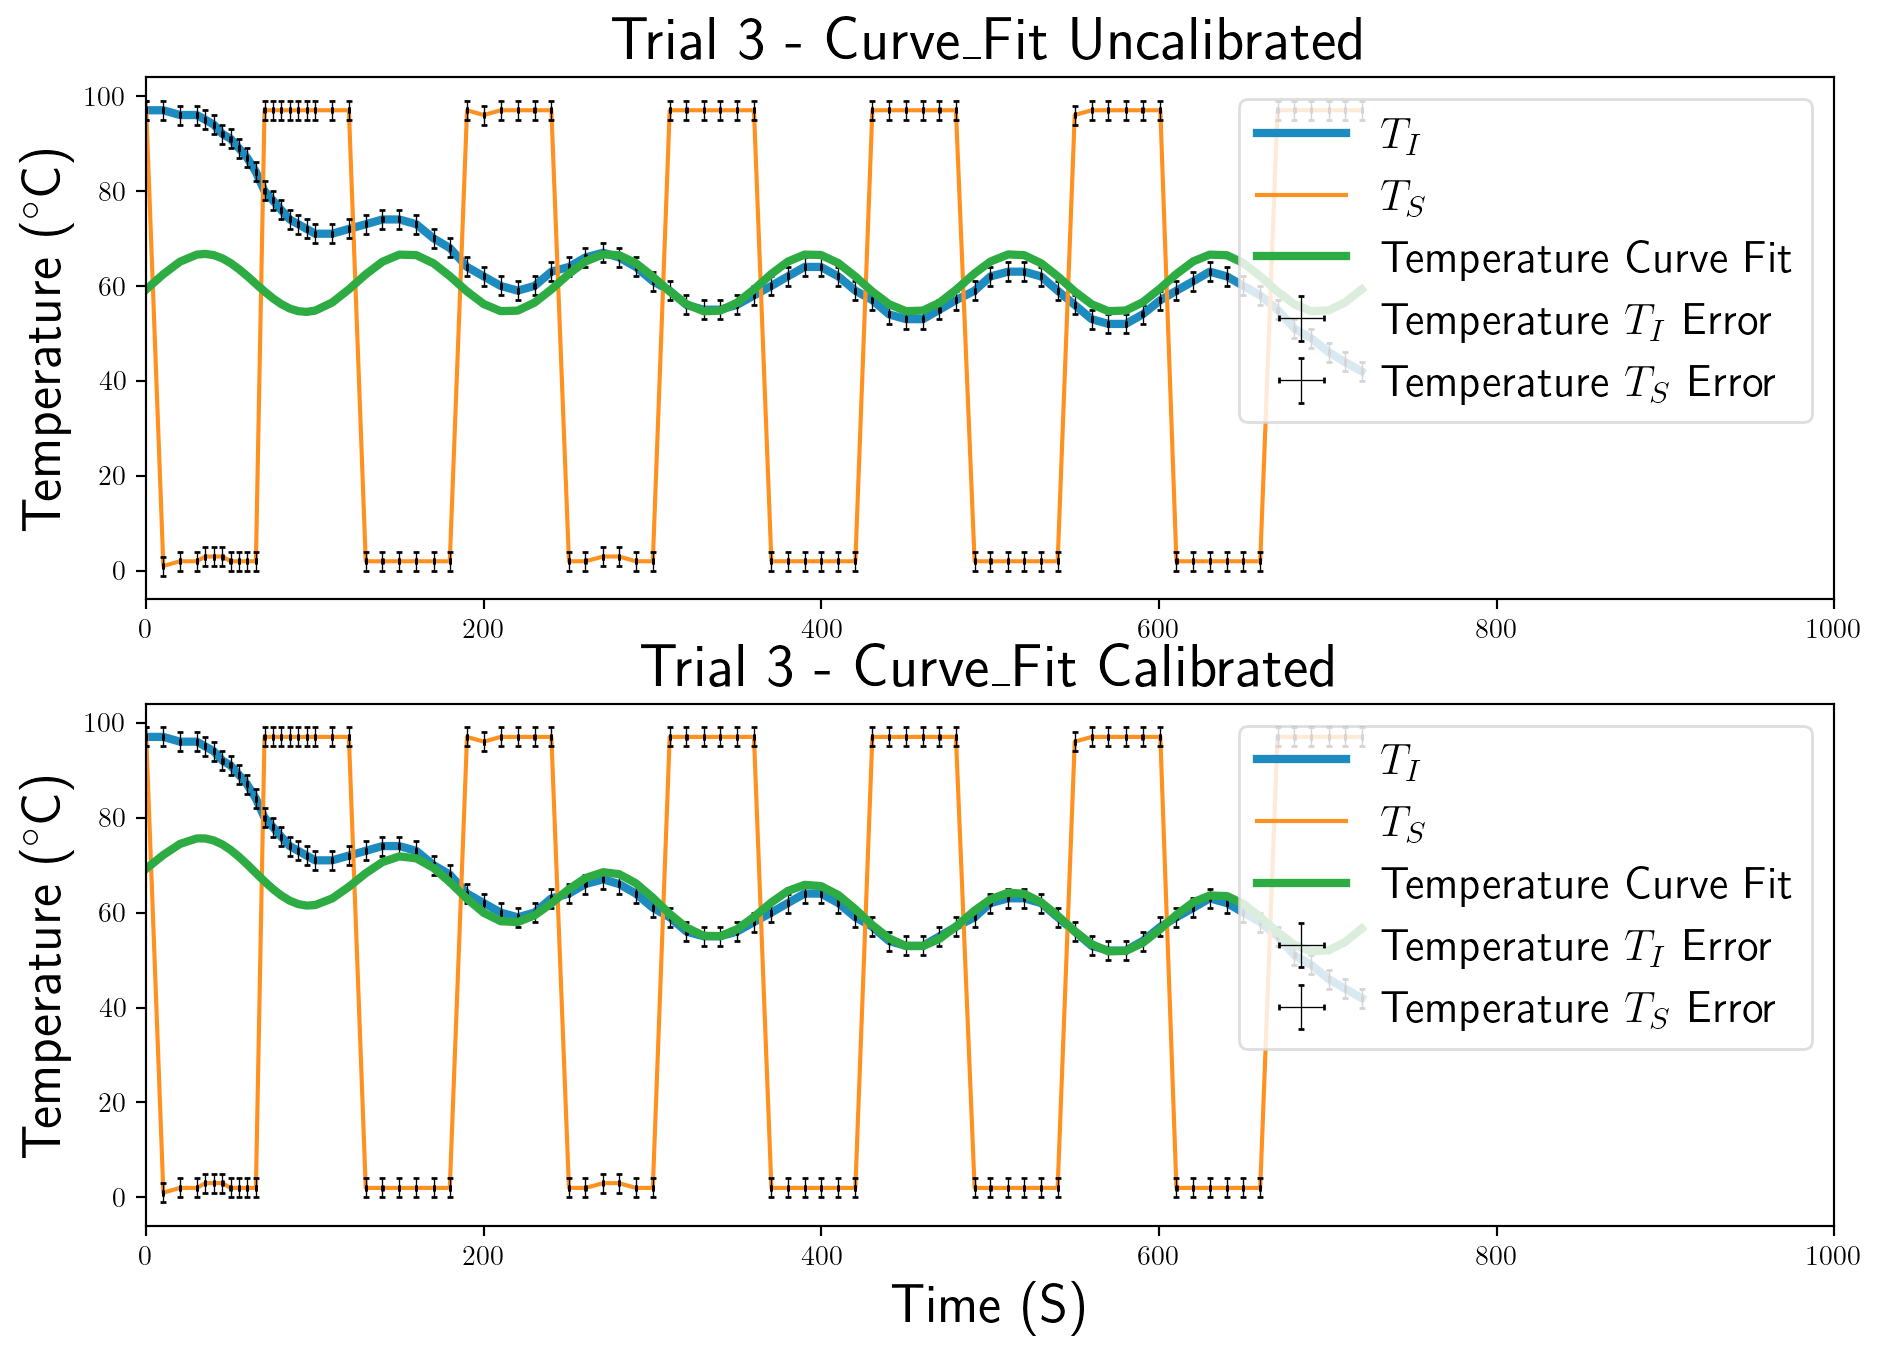
\includegraphics[width=3.7in]{calibration comparison.png}
        \caption*{[Figure 1] The comparison of curve fitting with and without calibration. This is an excerpt of the final data, used to show the process of data fitting.}
    \end{figure}

\vspace{-20pt}

    \begin{figure}[H]
        \hspace{-5pt}
        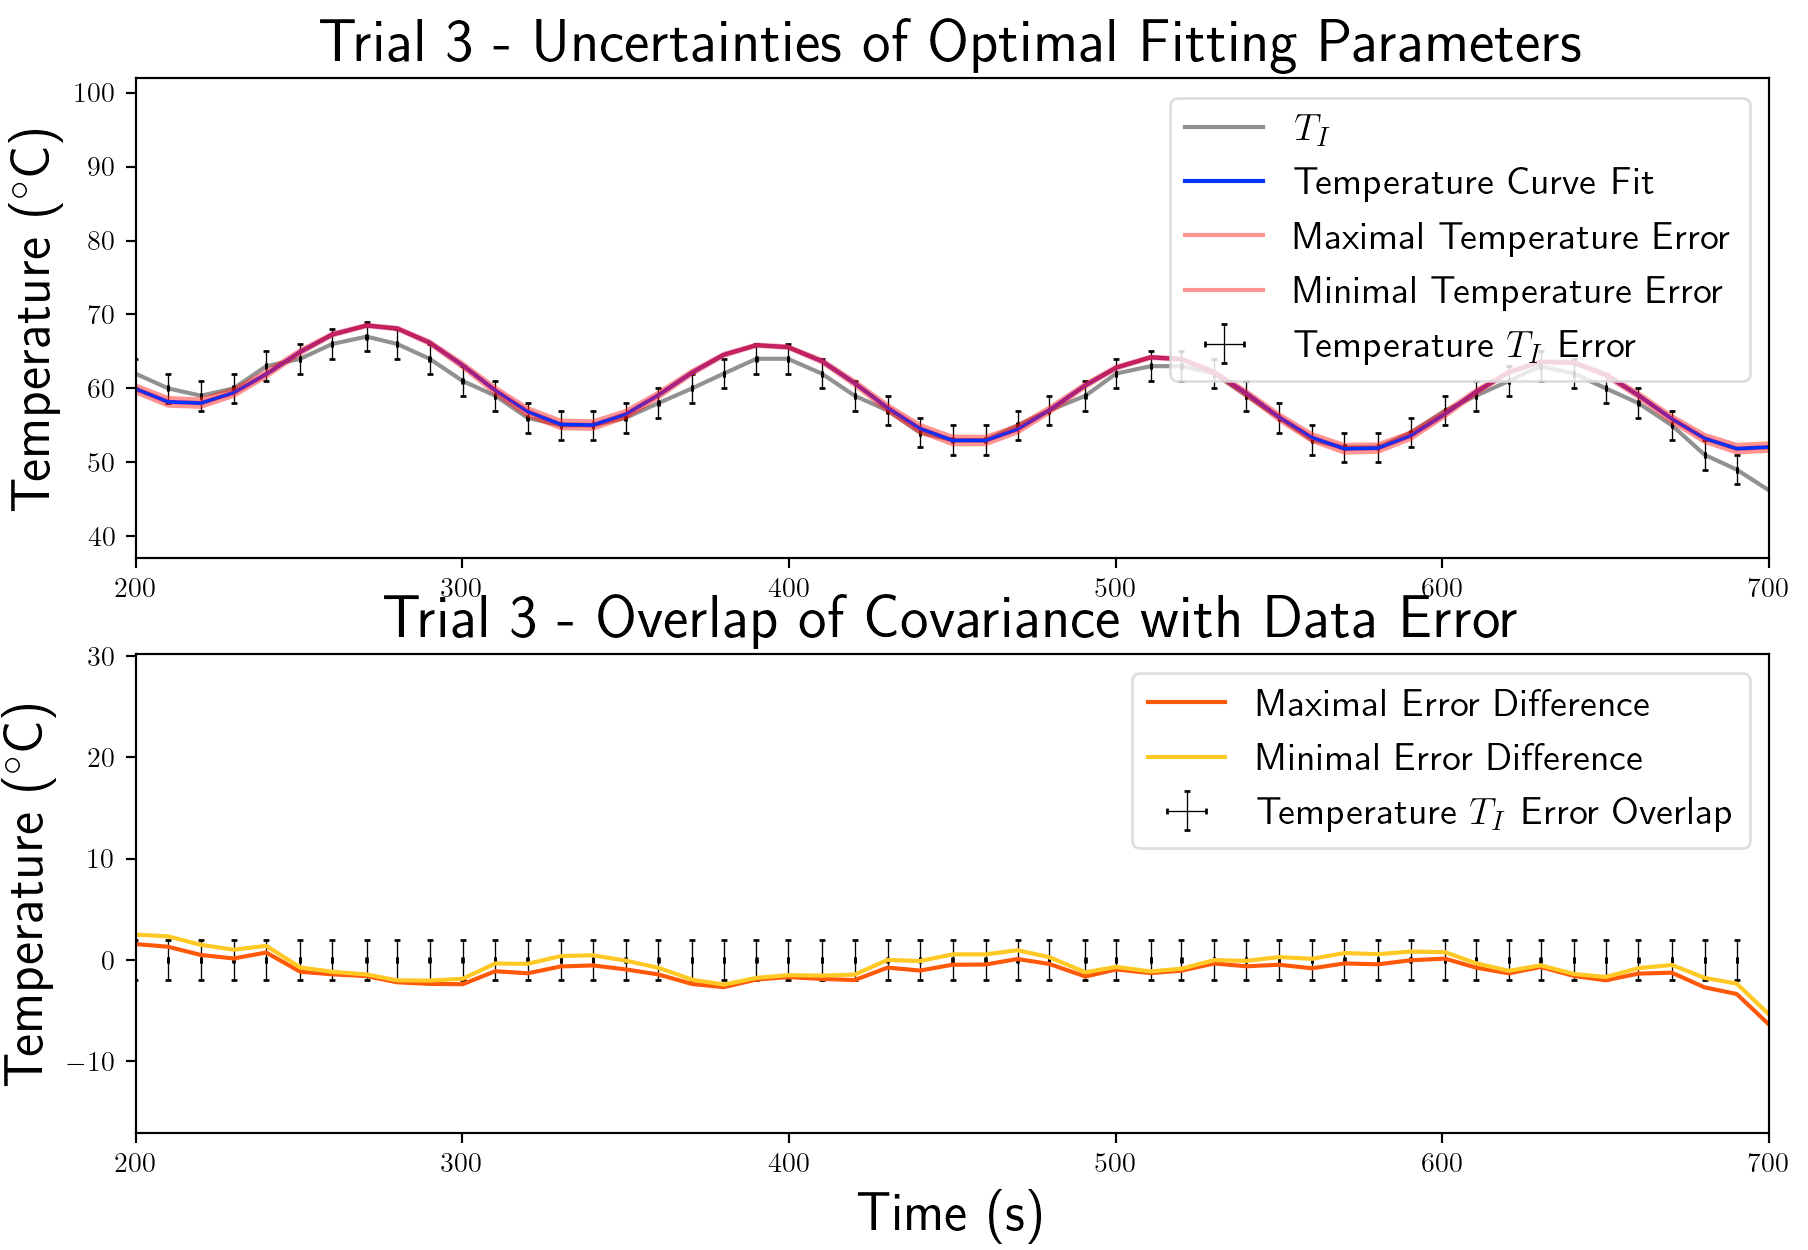
\includegraphics[width=3.85in]{uncertainty example.png}
        \caption*{[Figure 2] An instance of the uncertainty overlap observed while curve fitting. This is taken from Trial 3, from the final dataset to show how effective the covariance determination was.}
    \end{figure}

\end{multicols}

\vspace{0pt}

    \begin{figure}[H]
        \centering 
        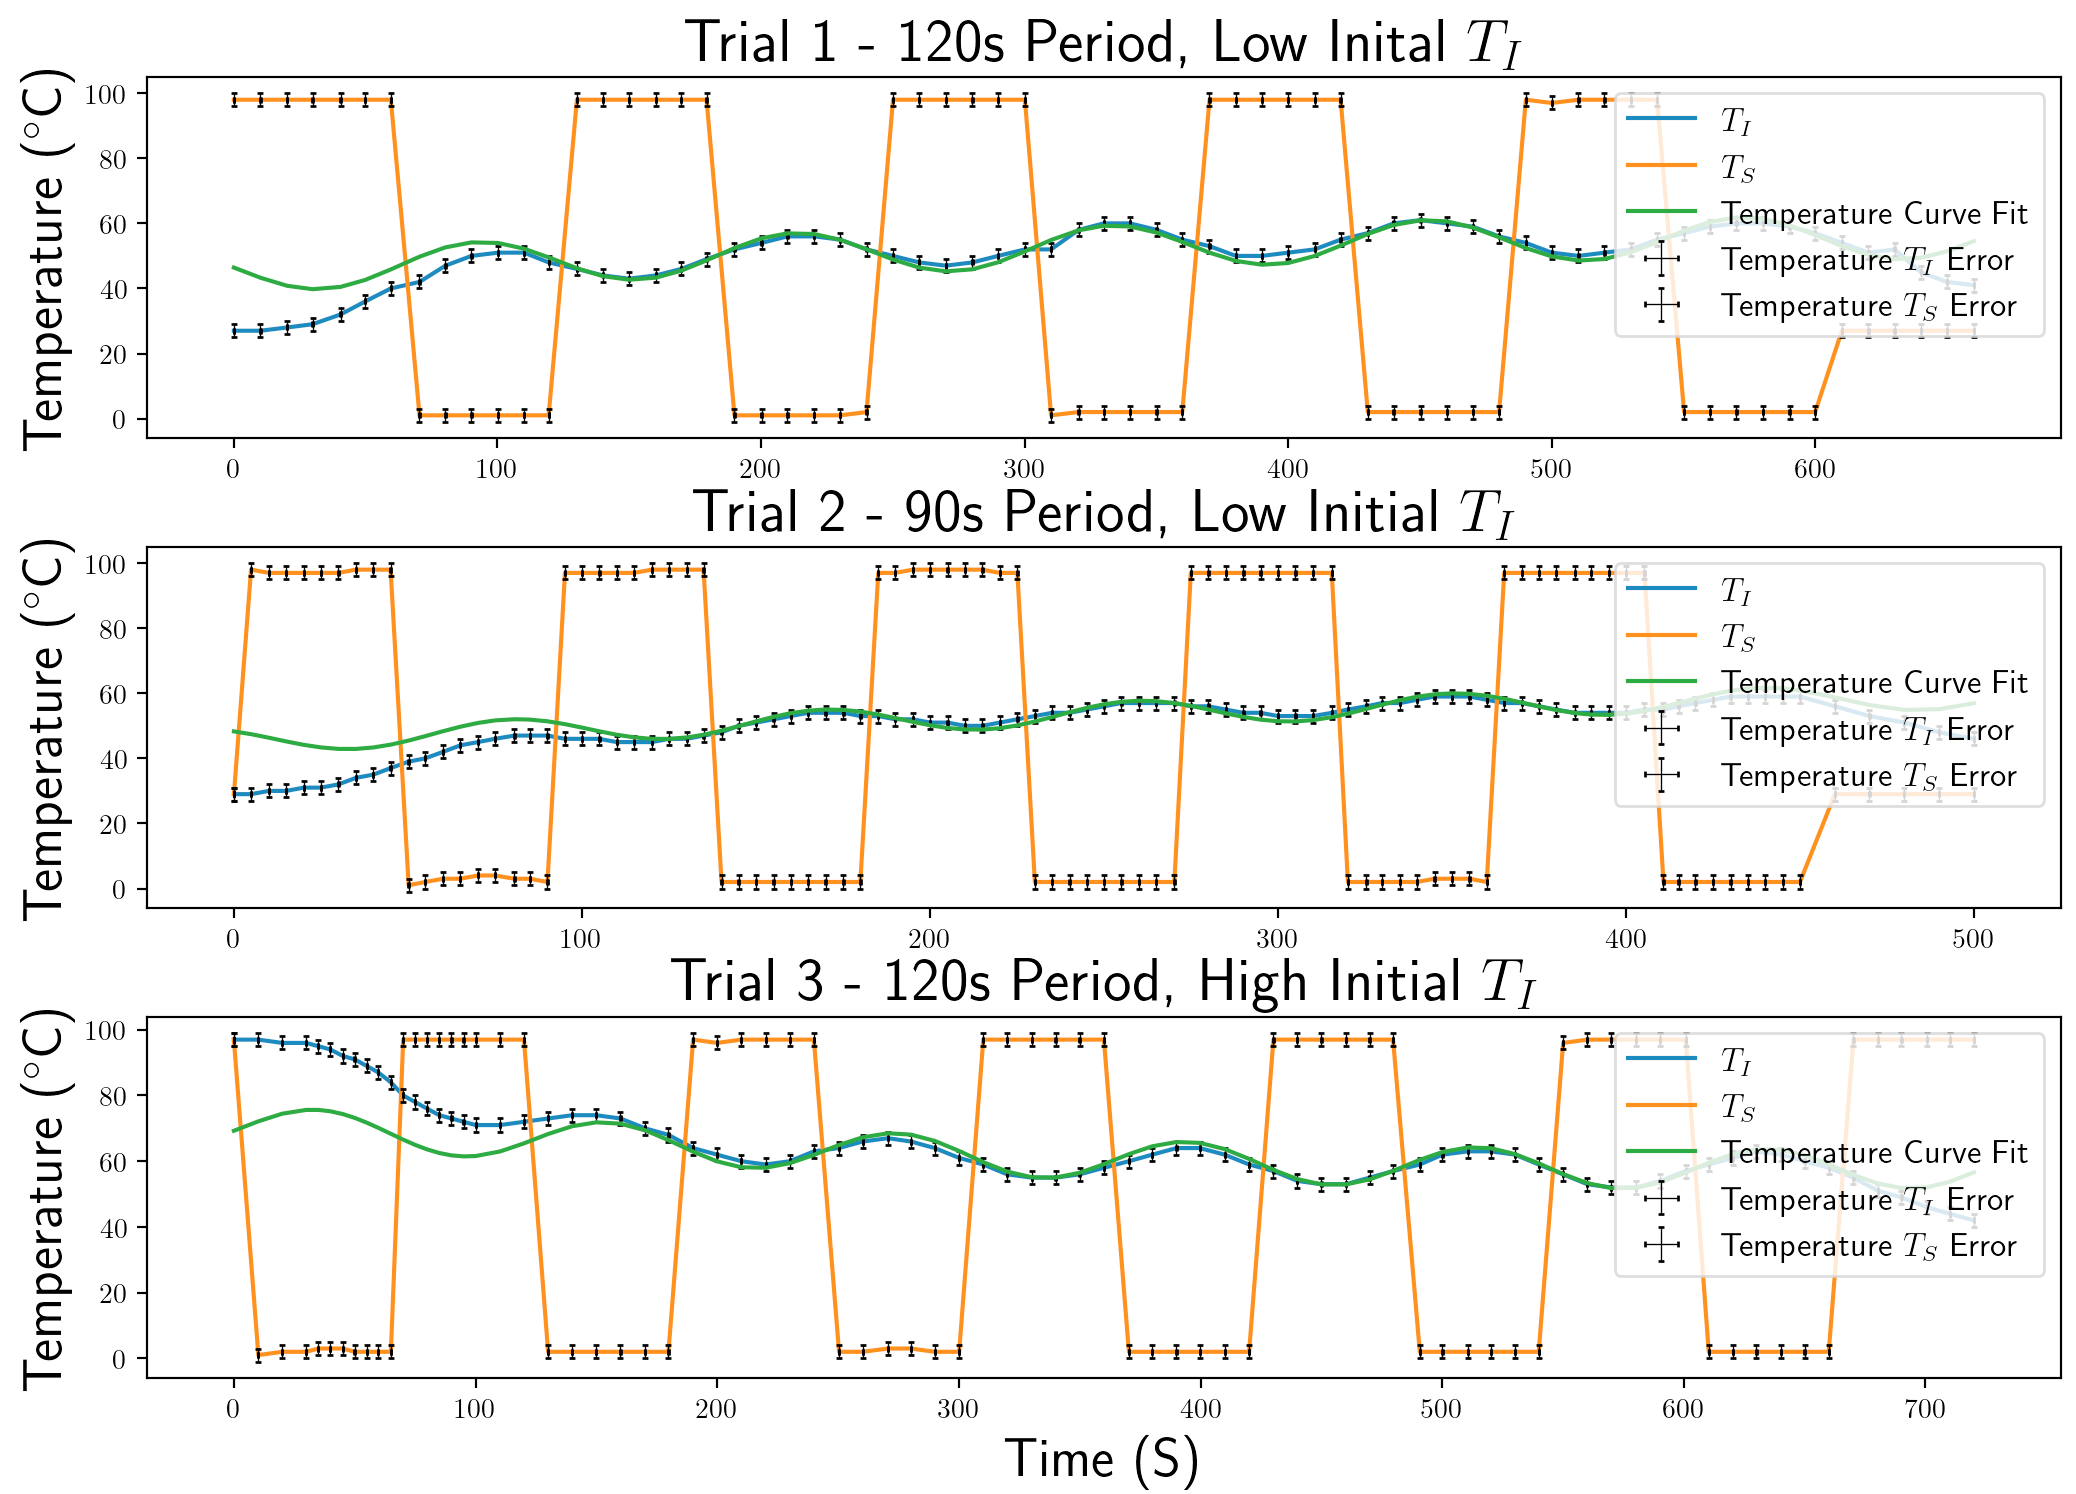
\includegraphics[width=5.5in]{data plots.png}
        \caption*{[Figure 3] The plotted data for all three trials, including uncertainties and calibrated curve fits. (Above) Trial 1, at 60s intervals with initial temperature $27^\circ$C. (Middle) Trial 2, at 45s intervals with initial temperature $29^\circ$C. (Below) Trial 3, again at 60s interval but with initial temperature $97^\circ$C. }
    \end{figure}

\vspace{-20pt}

    \begin{figure}[H]
        \centering 
        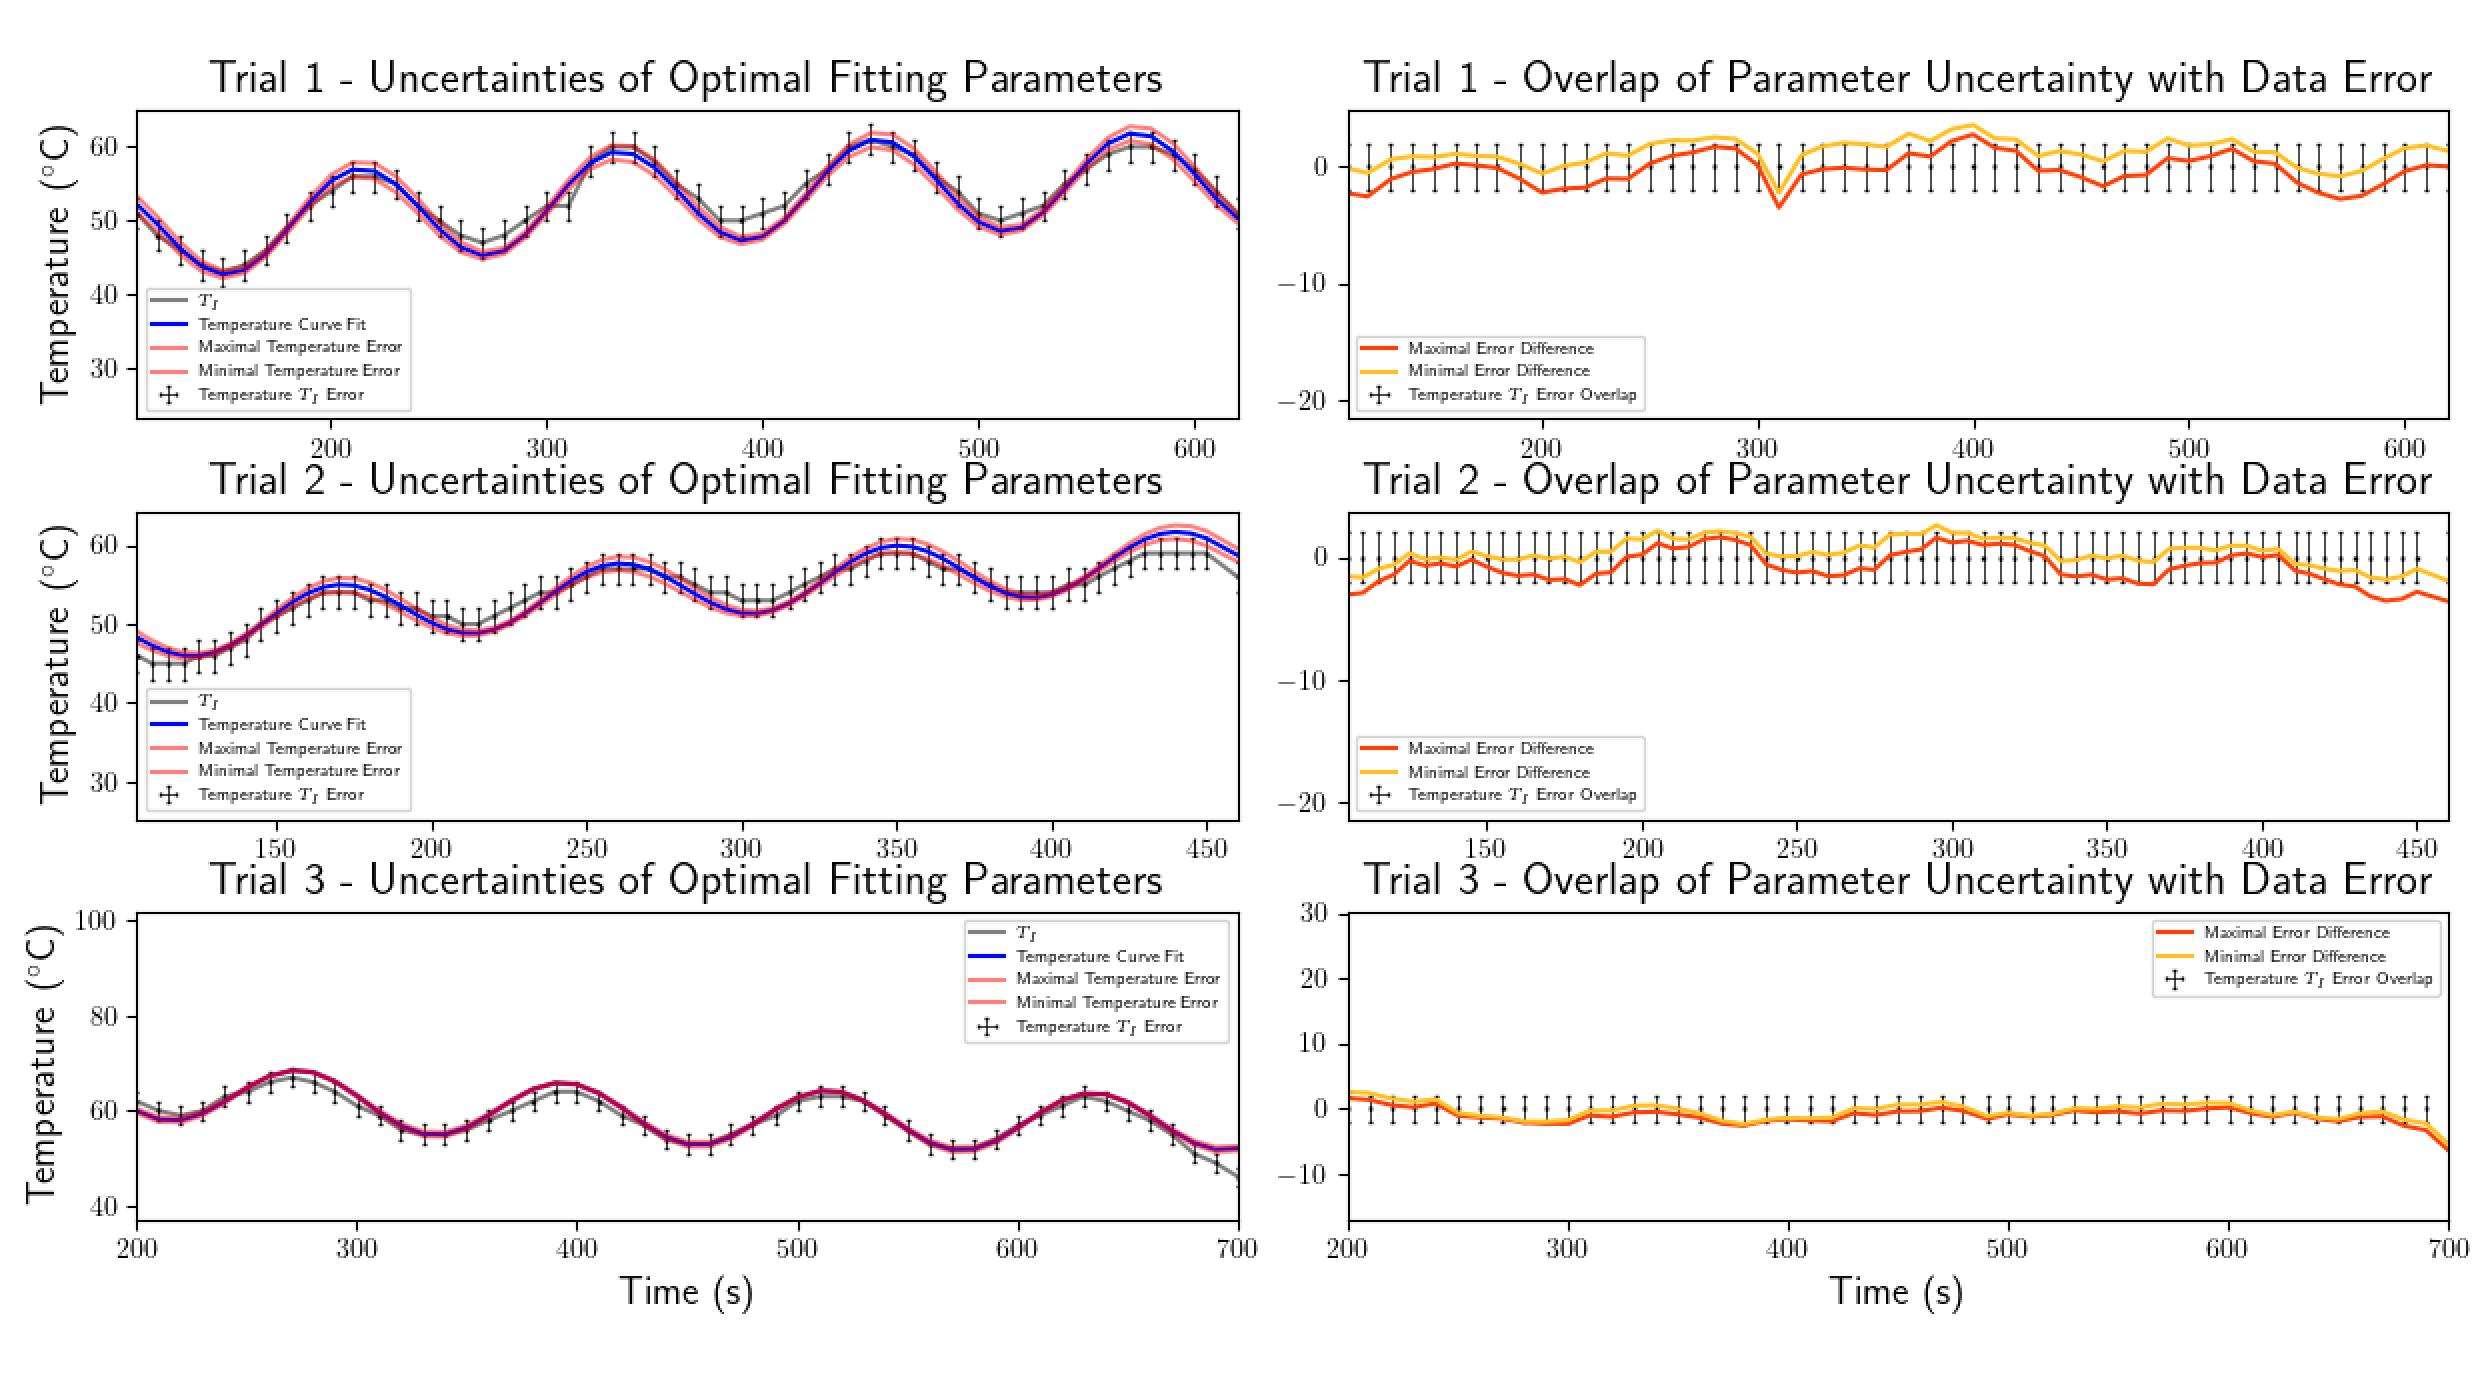
\includegraphics[width=7in]{uncertainty data.png}
        \caption*{[Figure 4] The visual overlap of the uncertainties recorded for acquired data and curve\_fit parameter covariances. The columns indicate trial number, while the rows indicate the `uncertainty of worst fit' (Left) and the distance between errors (Right). These plots were created by varying the optimal curve fit parameters with the maximum uncertainty of the covariances, and the comparing the uncertainty overlap with acquired data. }
    \end{figure}


    \begin{table}[H]
        \centering
        \resizebox{18cm}{!}{
        \begin{tabular}{|c|c|c|c|c|c|}
                \hline
            Trial & Period (s) & Initial Temperature ($^\circ $C)& $m$ (mm$^2$/s) & Error in $m$ (mm$^2$/s)& $\chi^2$ Fit Quality (\%)\\
                \hline
            1 & 120 & 27 & 0.092 & $\pm$ 0.002 & 0.99\\
                \hline
            2 & 90 & 29 & 0.14 & $\pm$ 0.01 & 0.99 \\
                \hline
            3 & 120 & 97 & 0.096 & $\pm$ 0.001 & 0.99 \\
                \hline
        \end{tabular}
        }
        \caption*{[Table 1] Results obtained for the computed values of the thermal diffusivity for each of the three trials. Included is the applied angular period, the intial temperature of the rubber, the curve\_fit computed value for the thermal diffusivity and uncertainty, and the quality of the $\chi^2$ fit.}   
    \end{table}





\end{document}